\documentclass[ ]{article}
\usepackage[usenames,dvipsnames]{xcolor} %used for font color
\usepackage[utf8]{inputenc} %useful to type directly diacritic characters
\usepackage[english]{babel}
\usepackage{listings}
\usepackage{tcolorbox}
\usepackage[ ]{tikz}
\tikzset{ram grid/.style = {black!100, very thick}}
\tcbuselibrary{listings, skins}


\title{Revisão P2 de Estruturas de Dados \\ Dênio Duarte}
\author{Erickson G. Müller}

\begin{document}

\definecolor{codebg}{HTML}{333333}
\definecolor{codetext}{HTML}{ffffff}
\definecolor{codegreen}{HTML}{57db0b}
\definecolor{codeorange}{HTML}{f78e05}
\definecolor{codered}{HTML}{f7052d}
\definecolor{codeshadow}{HTML}{432fa3}

\lstdefinestyle{codestyle}{
	basicstyle =  \color{codetext},
	language = C,
	keywordstyle = \color{codeorange}\bf,
	tabsize = 8
}
\newtcblisting{mylist}{
      enhanced,   %%% needed for shadow
      arc=5mm,
      top=2mm,
      bottom=2mm,
      left=2mm,
      right=10mm,
      boxrule=0pt,
      colback=codebg,
      shadow={1mm}{-1mm}{0mm}{fill=codeshadow,
                      opacity=0.5},             %%% here for shadow  and adjust as you like
      listing only,
      listing options={style=codestyle},
      hbox
}
%\lstset{style=codestyle}

\maketitle

\section{Conteúdos}
\begin{enumerate}
	\item Alocação Dinâmica de Memória
	\item Lista Simplesmente Encadeada
	\item Lista Duplamente Encadeada
	\item Filas e Pilhas
\end{enumerate}
\pagebreak
\section{Alocação Dinâmica de Memória}
	A Alocação Dinâmica de Lista Encadeada na Memória segue os seguintes passos:
	\begin{enumerate}
		\item Alocação de memória
		\item Colocar os valores no espaço alocado e NULLificar as variáveis ponteiras
		\item Encadeamento
	\end{enumerate}
\section{Estudo de Código}
	Desenvolver uma lista encadeada com alocação dinâmica é uma receita de bolo, para isso, iremos analisar cada etapa do código abaixo, que imprime uma sequência de pontos cartesianos.
	
	\begin{mylist}
#include <stdio.h>
#include <stdlib.h>

struct tpoint{
	int x,y;
	struct tpoint *next;
};
typedef struct tpoint tpnt;

int main(){
	tpnt *p, *aux, *first = NULL;
	int i;
	for(i=1;i<=10;i++){
		p = (tpnt*)malloc(sizeof(tpnt));
		
		p->x=i;
		p->y=i+10;
		
		if(first==NULL){
			first = p;
			aux = p;
		}
		else{
			aux->next = p;
			aux = p;
		}
	}
	
	for(aux=first;aux!=NULL;aux=aux->next){
		printf("(%d,%d)\n", aux->x,aux->y);
	}
	
	if(first!=NULL){
		aux=first;
		while(aux->next!=NULL){
			p = aux;
			aux = aux->next;
			free(p);
		}
		free(aux);
		first=NULL;
	}
	return 0;
}
	\end{mylist}
\section{Definir a Estrutura}
\begin{minipage}{8 cm}
	\begin{mylist}
struct tpoint{
	int x,y;
	struct tpoint *next;
};
typedef struct tpoint tpnt;
	\end{mylist}		
\end{minipage}
\begin{minipage}{8 cm}
	\begin{enumerate}
	\item Variáveis usadas nos itens dentro da lista
	\item Ponteiro *next, que apontará para o próximo da lista
	\item Atribuir um apelido para essa struct
	\end{enumerate}
\end{minipage}
\section{free\_memory \& *ins\_end}
	Antes de criarmos a função main, podemos inserir no código uma função para liberar o espaço de memória ou para fazer modificações na lista encadeada, como incluir novo item no meio da lista. Essas duas funções não estão presentes neste código e serão apresentadas ao final da explicação.
\section{Criar Variáveis Ponteiros}
\begin{minipage}{8 cm}
	\begin{mylist}
int(main){
	tpnt *p;
	tpnt *aux;
	tpnt *first = NULL;
	\end{mylist}
\end{minipage}
\begin{minipage}{8 cm}
	\begin{enumerate}
		\item *p - aponta para o item
		\item *aux - aponta para várias coisas ao mesmo tempo
		\item *first - se for NULL (first = p)
	\end{enumerate}
\end{minipage}

\section{Criar um Loop de Encadeamento}
	\begin{mylist}
	int i;
	for(i=1;i<=10;i++){
		p = (tpnt *)malloc(sizeof(tpnt)):

		p->x=i;
		p->y=i+10;
		
		if(first == NULL){
			first = p;
			aux = p;
		}
		else{
			aux->next = p;
			aux = p;
		}
	}
		
	\end{mylist}
	A primeira ação do loop é alocar espaço na memória através da linha:\begin{mylist}		p = (tpnt *)malloc(sizeof(tpnt)\end{mylist}\\
	Essa função vai designar um único espaço na memória para alterar suas variáveis conforme a iteração no loop. Assim, o programa fica mais leve na memória primária.\\
	\\
	Lembrando as três etapas do encadeamento:
	\begin{enumerate}
	\item \textbf{Alocação de memória}
	\item Colocar os valores no espaço alocado e NULLificar as variáveis ponteiras
	\item Encadeamento \vspace{1 cm} \\
	\begin{huge}
	RAM
	\end{huge}
	\end{enumerate}
	
	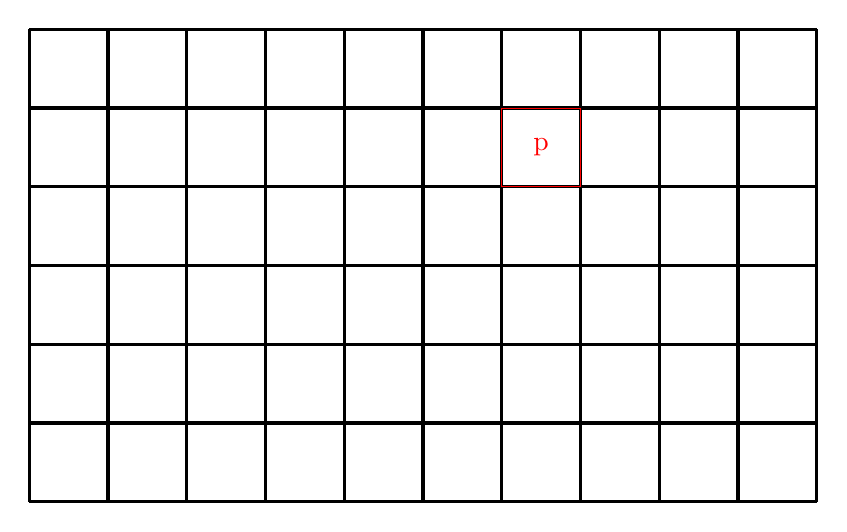
\begin{tikzpicture}
		\draw[ram grid,step=1.0cm] (0,0) grid (10,6);
		\draw[red] (6,4) rectangle(7,5) node[pos=0.5]{p};
	\end{tikzpicture}
	\\
	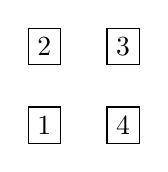
\begin{tikzpicture}
		\path
		(0,0) node [shape = rectangle,draw]{1}
		(0,1) node [shape = rectangle,draw]{2}
		(1,1) node [shape = rectangle,draw]{3}
		(1,0) node [shape = rectangle,draw]{4};		
	\end{tikzpicture}
	\\
	O código abaixo serve para atribuir valores às variáveis atuais. Pode ser de diversas formas diferentes.
	\begin{mylist}
		p->x = i;
		p->y = i + 10;
	\end{mylist}
	Em seguida vamos encadear a lista:
	\begin{mylist}
		if(first == NULL){
			first = p;
			aux = p;
		}
		else{
			aux->next = p;
			aux = p;
		}
	\end{mylist}
	O primeiro bloco é chamado quando a lista está vazia. Ele aponta o elemento $p$ como first e o $aux$ apontando para o próprio elemento. Inicialmente, todos apontam para a mesma região alocada.\\
	Dentro do else, $aux$ deve apontar sempre para a \textbf{região anterior} àquela a ser alocada, or isso que $aux->next = p$ antes de $aux = p$.\\
	\subsection{Como está a variável p em cada linha do loop}
	\begin{minipage}{8cm}
		\begin{mylist}
1 for(i=1;i<=10;i++){
2 	p = (tpnt*)malloc(sizeof(tpnt));
3		
4	p->x=i;
5	p->y=i+10;
6
7	if(first==NULL){
8		first = p;
9		aux = p;
10	}
11	else{
12		aux->next = p;
13		aux = p;
14	}
15 }
	
		\end{mylist}
	
	\end{minipage}
	
	
\section{Função para Printar as Coordenadas}
	\begin{mylist}
	for(aux=first; aux != NULL; aux = aux->nex){
		printf("(%d,%d)\n", aux->x,aux->y):
	}
	\end{mylist}
\end{document}